\documentclass[tikz]{standalone}
\usepackage{pgfplots}
\pgfplotsset{compat=1.17}
\begin{document}
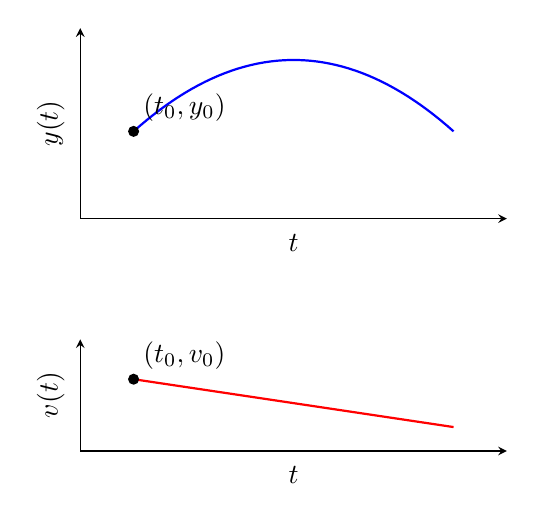
\begin{tikzpicture}
    \begin{axis}[
        name=pos,
        width=7cm, height=4cm,
        axis lines=left,
        xlabel={$t$}, ylabel={$y(t)$},
        xmin=0, xmax=4, ymin=0, ymax=6,
        xtick=\empty, ytick=\empty,
        ]
        \addplot[domain=0.5:3.5, samples=50, blue, thick] {5 - 1*(\x - 2)^2};
        \node[above right] at (axis cs:0.5, 2.75) {$(t_0, y_0)$};
        \fill (axis cs:0.5, 2.75) circle (2pt);
    \end{axis}
    \begin{axis}[
        name=vel,
        at={(pos.below south)}, yshift=-1cm,
        anchor=north,
        width=7cm, height=3cm,
        axis lines=left,
        xlabel={$t$}, ylabel={$v(t)$},
        xmin=0, xmax=4, ymin=-3, ymax=4,
        xtick=\empty, ytick=\empty,
    ]
        \addplot[domain=0.5:3.5, samples=2, red, thick] {2 - 1*(\x)};
        \node[above right] at (axis cs:0.5, 1.5) {$(t_0, v_0)$};
        \fill (axis cs:0.5, 1.5) circle (2pt);
    \end{axis}
\end{tikzpicture}
\end{document}
